\documentclass[12pt]{article}
\usepackage[UTF8]{ctex}
\usepackage{graphicx}
\usepackage{amsmath}
\usepackage{amsfonts} 


\begin{document}

\section{多模态大语言模型的训练}

\begin{figure}[ht]
    \centering
    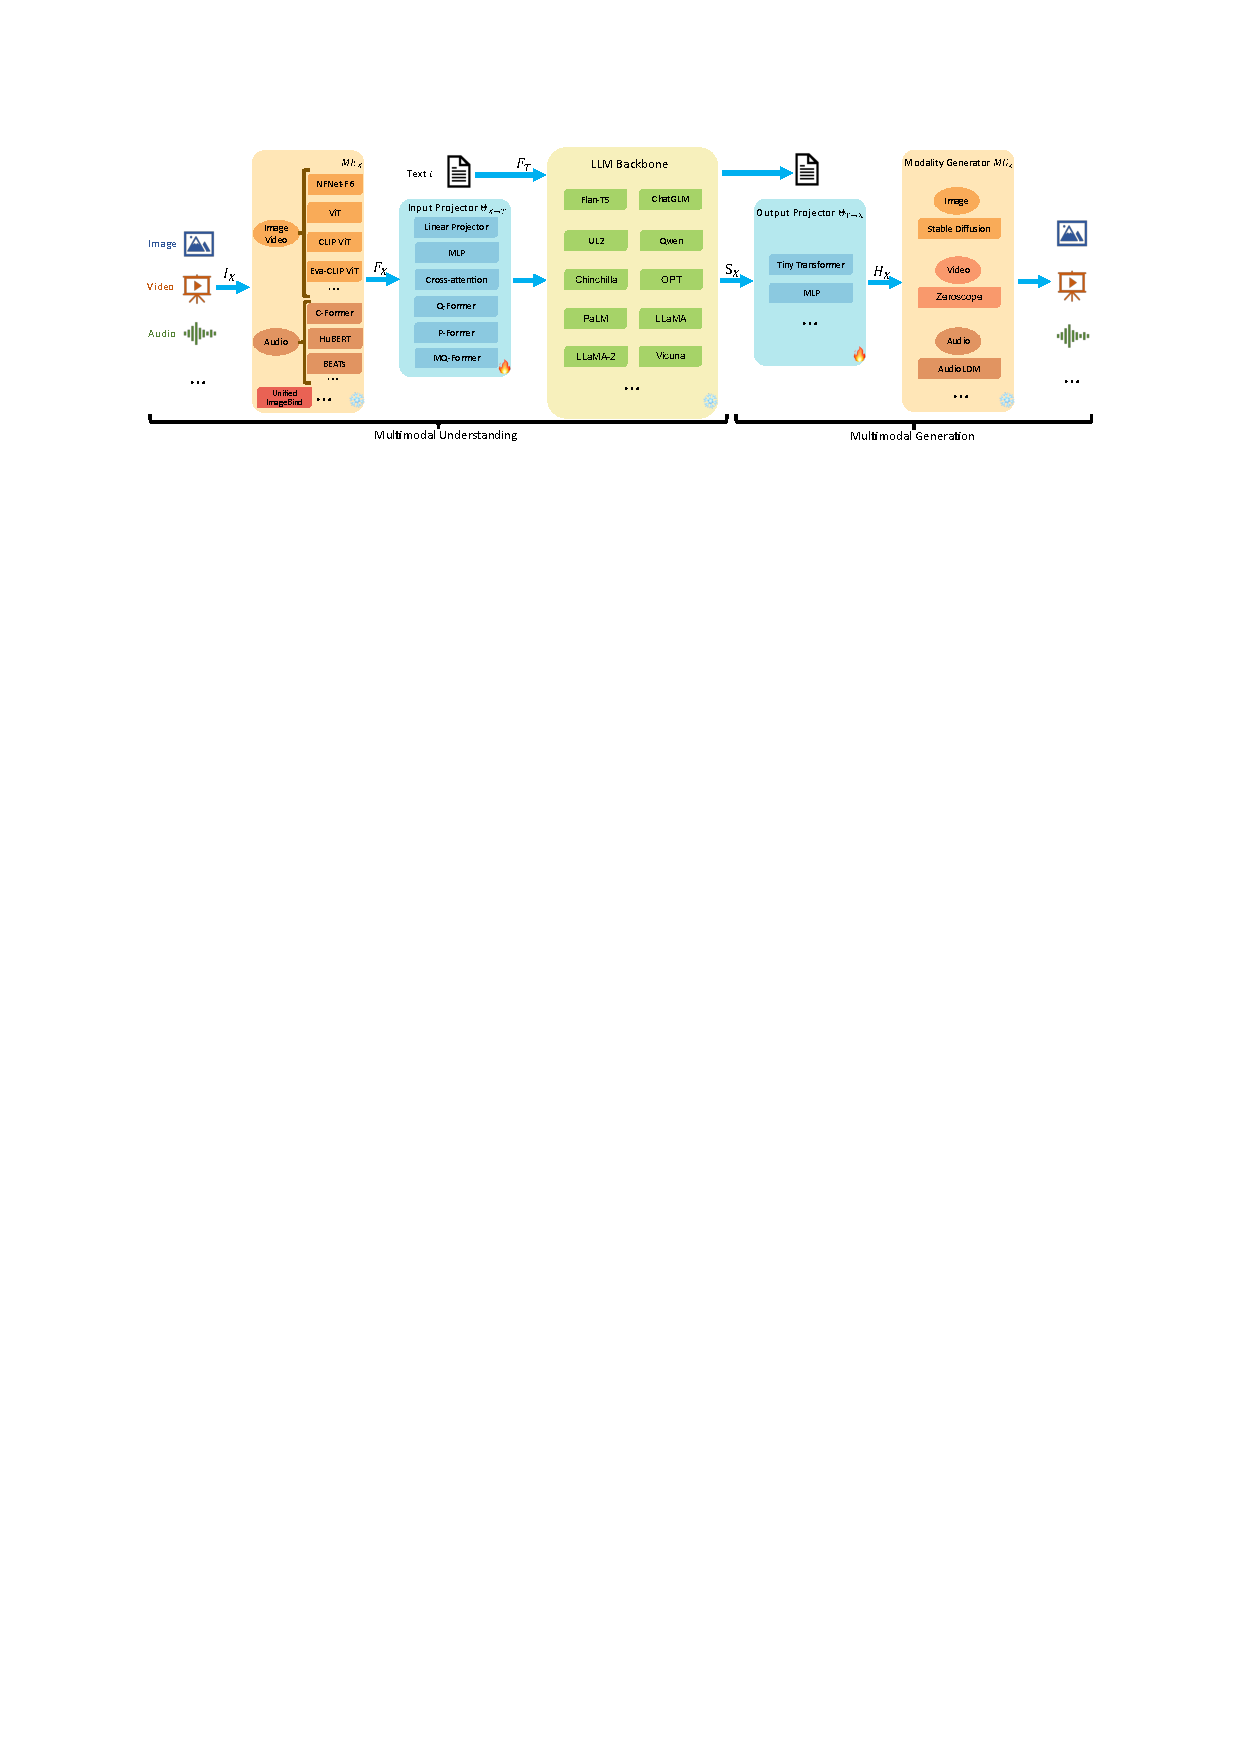
\includegraphics[width=1\textwidth, trim = 50 650 50 50]{MMLLM.pdf}
    \caption{MM-LLMs结构}
\end{figure}

在训练期间,多模态编码器(Modality Encoder)、LLM主干(LLM Backbone)和多模态生成器(Modality Generator)通常保持冻结状态。主要的优化重点在于输入和输出投影器(Input and Output Projectors)。由于投影器是轻量级组件,MM-LLMs中可训练参数的比例相对于总参数量显著较小(通常约为2\%)。总参数量取决于MM-LLMs中核心LLM的规模。因此,MM-LLMs可以高效训练以支持各种多模态任务。

\subsection{训练常用多模态数据集}

通常利用X-Text数据集,训练输入和输出投影器,通过优化预定义的目标来实现各种模态之间的对齐。X-Text数据集包括图文(Image-Text)、视频文本(Video-Text)和音频文本(Audio-Text),其中图文数据集分为两种类型:图文对(例如, )和交织的图文语料库(例如,)。X-Text数据集的详细信息见表3。


\begin{figure}[ht]
    \centering
    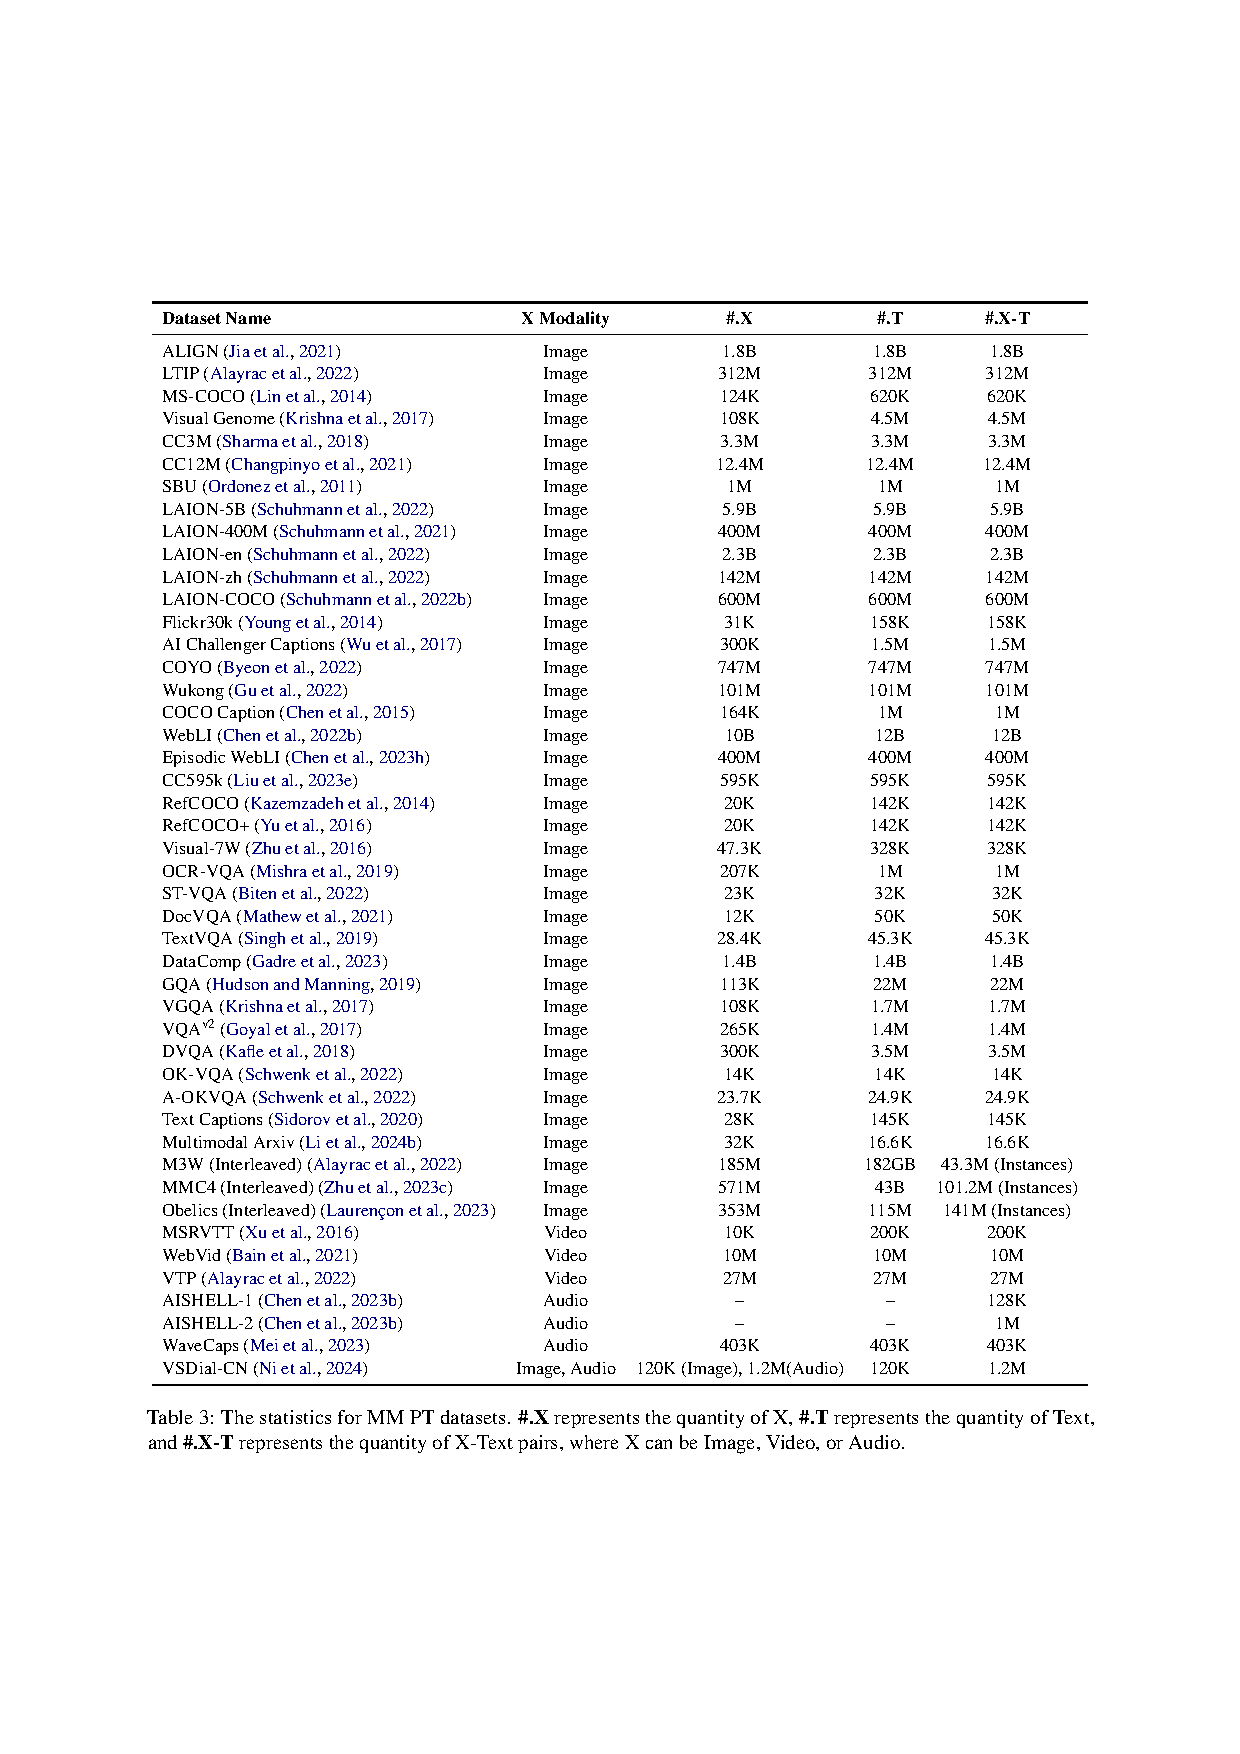
\includegraphics[width = 0.9\textwidth, trim = 50 150 50 50]{MMLLM_Dataset.pdf}
   
\end{figure}

\subsection{数据预处理}

数据预处理的目标是将原始的多模态数据(如文本、图像、视频、音频等)转换为模型能够理解和处理的格式,同时去除噪声、标准化数据,以提高训练效率和模型性能。

文本数据预处理:文本数据预处理包括分词、去除停用词、小写化和正则化等步骤,将文本数据标准化为更容易处理的形式。分词(Tokenization)是将文本分割为单词或子词的过程,如WordPiece和BPE等方法常用于此任务。为了减少无用数据,去除停用词和小写化文本是常见的预处理步骤。文本编码(如Word2Vec、GloVe)将分词后的文本转换为数值形式,以便输入模型。此外,遮盖(Masking)技术用于自监督学习任务,通过随机遮盖部分词汇,使模型学会预测这些词汇。

图像数据预处理:图像数据的预处理主要包括尺寸调整、归一化和数据增强等步骤。尺寸调整(Resizing)确保图像输入的统一格式,如调整为224x224像素。归一化(Normalization)是通过将像素值标准化为固定范围(如0到1),减少输入数据的差异。数据增强技术(Data Augmentation)如随机裁剪、旋转和翻转,可以增加数据的多样性,防止模型过拟合。在一些情况下,还会使用预训练卷积神经网络(如ResNet、VGG)进行特征提取,以便将图像转换为特征向量。

视频数据预处理:视频数据预处理相较于图像更复杂,涉及时间维度的操作,如帧提取和时间同步。帧提取(Frame Extraction)通常按照固定帧率从视频中提取连续或关键帧,以便后续处理。时间同步和对齐用于确保视频片段与文本或字幕正确匹配。此外,视频特征提取常用3D卷积网络或时空特征网络(如I3D、SlowFast)来获取视频的时空特征。视频预处理中的数据增强包括帧的尺寸调整、归一化以及时间维度的调整(如速度变化)。

音频数据预处理:音频数据预处理步骤包括采样率调整、去噪和特征提取。统一采样率(如16kHz)可以确保数据一致性,去噪处理用于去除背景噪声和不必要的频率成分。特征提取是音频预处理的重要部分,通过生成梅尔频谱图(Mel-Spectrogram)或梅尔频率倒谱系数(MFCC)等特征,将音频信号转换为时间-频率表示。此外,音频信号通常会被分割为短时间窗口(如25ms),以捕捉语音的短时特征。

多模态数据对齐:多模态数据对齐是多模态预处理的关键步骤,确保不同模态之间的语义和时序一致性。语义对齐涉及匹配语义相关的图像和文本,确保图文配对数据的正确性。时序对齐则用于视频-文本或音频-文本的对齐,确保模态之间在时间上的同步。此外,对齐后的数据需要进行验证,可能采用人工或自动评估手段,以确保对齐的准确性,为后续训练提供高质量的数据输入。

\subsection{损失函数设计}

\subsubsection{单模态损失}
这些损失函数用于优化单个模态的数据表现。例如,对于图像和文本分别使用的分类、生成等任务损失。
\begin{description}
    \item[文本模态的损失函数] 文本模态的损失函数主要用于自然语言处理任务,如文本分类、语言建模和文本生成等。常见的损失函数包括交叉熵损失、语言模型损失和对比损失。交叉熵损失(Cross-Entropy Loss)用于文本分类和生成任务,衡量预测分布与真实分布之间的差异,公式为:
    
  \[
\text{Cross-Entropy Loss} = -\sum_{i=1}^{C} y_i \log(\hat{y}_i)
\]


    其中,\( y_i \) 是真实标签,\( \hat{y}_i \) 是预测的概率。对于语言建模任务,语言模型损失通过最大化被遮盖词或下一个词的预测概率,使模型更好地理解和生成自然语言。对比损失(Contrastive Loss)则用于文本相似度和匹配,通过拉近相似文本对,推远不相似对,常见形式为:
    \[
\text{Contrastive Loss} = -\log \frac{\exp(\text{sim}(h_1, h_2))}{\sum_{j=1}^{N} \exp(\text{sim}(h_1, h_j))}
\]
其中,\( \text{sim}(h_1, h_2) \) 表示相似度,如余弦相似度。
    \item[图像模态的损失函数] 
    
图像模态的损失函数用于图像分类、检测和生成任务,常见的有交叉熵损失、均方误差、生成对抗损失和IoU损失。交叉熵损失在图像分类任务中,通过最小化预测与真实类别的分布差异来优化模型。均方误差(Mean Squared Error, MSE)用于图像重建和去噪,衡量预测图像与真实图像像素间的平方差距,公式为:

\[
\text{MSE} = \frac{1}{N} \sum_{i=1}^{N} (x_i - \hat{x}_i)^2
\]

其中,\( x_i \) 和 \( \hat{x}_i \) 分别是真实值和预测值。生成对抗损失(GAN Loss)用于生成对抗网络,通过生成器和判别器的对抗训练,使生成图像更逼真:

\[
\text{GAN Loss} = \mathbb{E}_{x \sim p_{\text{data}}}[\log D(x)] + \mathbb{E}_{z \sim p_z}[\log (1 - D(G(z)))]
\]

其中,\( D \) 是判别器,\( G \) 是生成器。IoU损失(Intersection over Union Loss)用于目标检测,通过最大化预测框和真实框的交集比,优化检测性能。



    \item[视频模态的损失函数] 视频模态的损失函数用于优化视频分类、动作识别、视频生成等任务,常见的有时间对比损失、交叉熵损失、序列预测损失和生成对抗损失。时间对比损失(Temporal Contrastive Loss)用于学习视频时序特征,通过对比学习提升视频帧或片段之间的时序一致性。它的典型形式是基于对比学习的损失,如 InfoNCE(Noise-Contrastive Estimation)损失:

    \[
    \text{Temporal Contrastive Loss} = -\log \frac{\exp(\text{sim}(h_t, h_{t+1}) / \tau)}{\sum_{j=1}^{N} \exp(\text{sim}(h_t, h_j) / \tau)}
    \]
 
    其中,\( \text{sim}(h_t, h_{t+1}) \) 表示当前帧 \( t \) 和下一帧 \( t+1 \) 的特征相似度,\( \tau \) 为温度参数。通过最大化连续帧的相似度,模型学习到时序信息。交叉熵损失(Cross-Entropy Loss)用于视频分类和动作识别任务,衡量预测类别与真实类别之间的差异。交叉熵损失的公式与文本模态相同。序列预测损失(Sequence Prediction Loss)用于视频生成或时序预测任务,常用的损失形式是均方误差(MSE),衡量预测帧与真实帧之间的误差:

    \[
    \text{Sequence Prediction Loss} = \frac{1}{T} \sum_{t=1}^{T} (x_t - \hat{x}_t)^2
    \]
 
    其中,\( x_t \) 是真实的第 \( t \) 帧,\( \hat{x}_t \) 是预测的第 \( t \) 帧。
    
    生成对抗损失(Generative Adversarial Loss)用于视频生成任务,通过生成器和判别器之间的对抗训练,使得生成的视频更加逼真。生成器的损失公式为:

    \[
    \text{GAN Loss} = \mathbb{E}_{x \sim p_{\text{data}}}[\log D(x)] + \mathbb{E}_{z \sim p_z}[\log (1 - D(G(z)))]
    \]
 
    其中,\( D \) 是判别器,判断输入是否为真实视频,\( G \) 是生成器,生成视频片段 \( G(z) \) 以欺骗判别器。
 \item[音频模态的损失函数]
 音频模态的损失函数用于语音识别、音频分类和语音合成等任务,常见的有CTC损失、交叉熵损失和L1/L2损失。CTC损失(Connectionist Temporal Classification Loss)特别适用于语音识别,允许输入和输出序列长度不匹配的情况,公式为:
 
 \[
 \text{CTC Loss} = -\log p(\mathbf{y} | \mathbf{x})
 \]
 
 其中,\( p(\mathbf{y} | \mathbf{x}) \) 是音频输入到文本输出的概率路径和。交叉熵损失常用于音频分类任务,通过优化预测的类别概率。L1/L2损失用于语音合成和去噪,衡量音频特征的误差,如L2损失的公式为:
 
 \[
 \text{L2 Loss} = \frac{1}{N} \sum_{i=1}^{N} (x_i - \hat{x}_i)^2
 \]
 
 对比学习损失也在音频特征学习中使用,通过学习有区分性的音频片段表示,提升音频检索和分类性能。
 

\end{description}
\subsubsection{多模态损失}

跨模态损失旨在优化多模态数据之间的关联,使得模型能够在共享的特征空间中理解和处理不同模态的输入。它通过惩罚不正确的跨模态映射或不一致的对齐,指导模型调整各模态之间的特征表示。

\begin{description}
    \item[对比损失(Contrastive Loss)] 

    对比损失是跨模态对齐任务中最常见的损失类型,用于学习不同模态之间的相似性。它通过拉近相关模态对的特征(如图文对),推远不相关模态对的特征,从而优化跨模态对齐效果。
    
    \[
    \text{Contrastive Loss} = -\log \frac{\exp(\text{sim}(h_{\text{img}}, h_{\text{text}}) / \tau)}{\sum_{j=1}^{N} \exp(\text{sim}(h_{\text{img}}, h_{\text{neg}_j}) / \tau)}
    \]
    
    - \( h_{\text{img}} \) 和 \( h_{\text{text}} \) 是图像和文本的嵌入表示。
    - \( \text{sim} \) 表示相似度函数(如余弦相似度)。
    - \( \tau \) 为温度参数,调整对比的敏感度。
    - 这个损失通过最大化正样本对(图文对)的相似度,最小化与负样本对的相似度。
    \item[匹配损失(Matching Loss)]

    匹配损失用于衡量模态之间的直接匹配程度,如图文或视频-文本对的直接相似性得分,通常通过余弦相似度或点积计算。
    
    \[
    \text{Matching Loss} = \sum_{i=1}^{N} \left[ -\text{sim}(h_{\text{img}_i}, h_{\text{text}_i}) + \frac{1}{M} \sum_{j=1}^{M} \text{sim}(h_{\text{img}_i}, h_{\text{neg}_j}) \right]
    \]
    
    - \( N \) 是正样本对的数量。
    - \( M \) 是负样本对的数量。
    - 这个损失惩罚正样本的相似度低于负样本,推动模型学习更准确的跨模态对齐。
    \item[互信息最大化损失(Mutual Information Maximization Loss)]
    \item[] 
    互信息最大化损失用于增强模态间的依赖性,通过最大化不同模态特征之间的互信息,使模型更好地学习跨模态关系。
    
    \[
    \text{Mutual Information Loss} = -\sum_{i=1}^{N} I(h_{\text{img}_i}; h_{\text{text}_i})
    \]
    
    - \( I(h_{\text{img}}; h_{\text{text}}) \) 表示图像和文本特征之间的互信息。
    - 互信息最大化能够捕捉复杂的跨模态关系,提升多模态表征学习的效果。
    \item[生成对抗损失(Generative Adversarial Loss)]

    在跨模态生成任务(如文本生成图像)中,生成对抗损失通过生成器和判别器的对抗学习,使得生成模态(如生成图像)与输入模态(如文本描述)保持一致。
    
    \[
    \text{GAN Loss} = \mathbb{E}_{x \sim p_{\text{data}}}[\log D(x)] + \mathbb{E}_{z \sim p_z}[\log (1 - D(G(z, h_{\text{text}})))]
    \]
    
    - 生成器 \( G \) 生成跨模态输出,判别器 \( D \) 判断其是否与真实数据一致。
    - 通过对抗训练,模型学会生成符合输入模态语义的输出。
    
\end{description}

\subsection{训练策略}
多模态大语言模型的训练策略是确保模型高效学习不同模态之间复杂关系的重要环节。训练策略直接影响模型的性能、泛化能力和计算效率。多模态模型常用的训练策略包括预训练-微调策略、协同训练、分布式训练与混合精度训练、数据增强策略以及参数高效微调策略。
\subsubsection{预训练-微调策略(Pre-training and Fine-tuning Strategy)}


预训练-微调策略是多模态模型训练的核心方法,通过两阶段的训练流程提升模型的泛化能力和任务表现。在预训练阶段,模型利用大规模未标注或弱标注的多模态数据进行自监督学习,学习不同模态之间的基础表示和对齐关系。常见的自监督任务包括遮盖语言模型(Masked Language Modeling, MLM)和图文对比学习。预训练的目标函数通常为自监督损失,例如MLM的损失为:

\[
\text{MLM Loss} = -\sum_{i=1}^{N} \log P(x_i | x_{mask})
\]

其中,\( x_{mask} \) 是部分被遮盖的输入文本,\( x_i \) 是被遮盖的词语。微调阶段,模型在特定任务数据集上进行有监督微调,以优化模型在目标任务上的表现,如视觉问答或图文生成,微调的损失通常是任务特定的有监督损失(如交叉熵损失)。这种策略能够快速适应多样化的下游任务,并充分利用预训练阶段学到的跨模态知识。

\subsubsection{协同训练(Co-training Strategy)}

协同训练策略通过联合优化多个模态或任务的损失函数,增强模型对跨模态关系的理解。在协同训练中,模型在处理单模态任务时,同时学习跨模态特征,从而提升整体性能。协同训练的损失函数通常为多任务损失的加权组合:

\[
\text{Total Loss} = \lambda_1 \mathcal{L}_{\text{text}} + \lambda_2 \mathcal{L}_{\text{image}} + \lambda_3 \mathcal{L}_{\text{cross-modal}}
\]

其中,\( \mathcal{L}_{\text{text}} \) 是文本任务的损失,\( \mathcal{L}_{\text{image}} \) 是图像任务的损失,\( \mathcal{L}_{\text{cross-modal}} \) 是跨模态对齐损失,权重 \( \lambda \) 控制不同任务的重要性。通过共享参数和联合损失优化,模型能更好地捕捉模态间的语义关系,并提高数据利用率,使得模型在多个任务上均表现优异。

\subsubsection{分布式训练与混合精度训练(Distributed and Mixed Precision Training)}

分布式训练与混合精度训练是提升模型训练效率的关键策略。分布式训练通过多个GPU或TPU同时工作,将模型的计算任务分配到多个设备上,从而显著加速训练过程;混合精度训练通过将部分计算转换为半精度(FP16),减少显存占用和计算量。分布式训练的优化过程通常采用数据并行策略,其损失函数的优化形式为:

\[
\mathcal{L}_{\text{total}} = \frac{1}{K} \sum_{k=1}^{K} \mathcal{L}_k
\]

其中,\( K \) 是并行设备的数量,\( \mathcal{L}_k \) 是第 \( k \) 个设备计算的损失。混合精度训练结合损失缩放(Loss Scaling)技术,调整损失函数的尺度,避免数值不稳定:

\[
\text{Scaled Loss} = \mathcal{L} \times \text{Scale Factor}
\]

此策略不仅提高了训练速度,还降低了对硬件资源的需求,使得大型多模态模型的训练变得更加可行和高效。

\subsubsection{数据增强策略(Data Augmentation Strategy)}

数据增强策略通过对输入数据进行随机变换,增加数据的多样性,从而提升模型的泛化能力和鲁棒性。这些变换包括图像的随机裁剪、旋转、颜色抖动,文本的同义词替换、随机删除词,音频的时间拉伸、噪声注入等。增强后的数据通过保持原始标签来扩充训练集,增强的损失函数形式为:

\[
\mathcal{L}_{\text{augmented}} = \frac{1}{N} \sum_{i=1}^{N} \mathcal{L}(f(x_i), y_i)
\]

其中,\( x_i \) 是增强后的输入样本,\( y_i \) 是其对应的标签。通过随机扰动输入,模型能够更好地应对数据中的噪声和变异,同时避免过拟合,确保训练过程的稳定性和泛化效果。

\subsubsection{参数高效微调策略(Parameter-Efficient Fine-tuning Strategy)}

参数高效微调策略专注于减少微调时需要更新的参数量,从而提升微调效率和降低计算成本。通过技术如LoRA(Low-Rank Adaptation)、Adapter Tuning和Prefix-Tuning,仅微调少量参数,而保留大部分预训练模型的参数不变。LoRA的微调损失函数通常包含对低秩参数的优化:

\[
\mathcal{L}_{\text{LoRA}} = \mathcal{L}_{\text{task}} + \lambda \|\mathbf{W} - \mathbf{W}_{\text{base}} - \mathbf{A}\mathbf{B}\|^2
\]

其中,\( \mathbf{W} \) 是微调后的权重,\( \mathbf{W}_{\text{base}} \) 是基础模型的权重,\( \mathbf{A} \) 和 \( \mathbf{B} \) 是低秩矩阵。通过只更新附加的低秩矩阵或适配器模块,这种策略有效减少了训练计算量,使得微调快速且节省资源,特别适合多任务或多领域的快速适应。

\end{document}